In this chapter a description of the houses and the inhabitants is given. The different kind of sensors are explained and an impression of the received data is given.

\section{Homes and persons}
In the homes of five different people sensors are installed. The floor-plan of these homes is for all residents the same and is shown in figure \ref{fig:floorplan}. There might be small differences of the locations of the sensors due to the personal arrangements of peoples personal belongings.
The persons that live in the homes are people that need healthcare on a regular basis, they are further able to live on their own. The amount of data collected differs for the different houses, but there is at least 63 days of data available for every house. An overview of the different houses is given in table \ref{table:houses}

\begin{figure}
\centering
 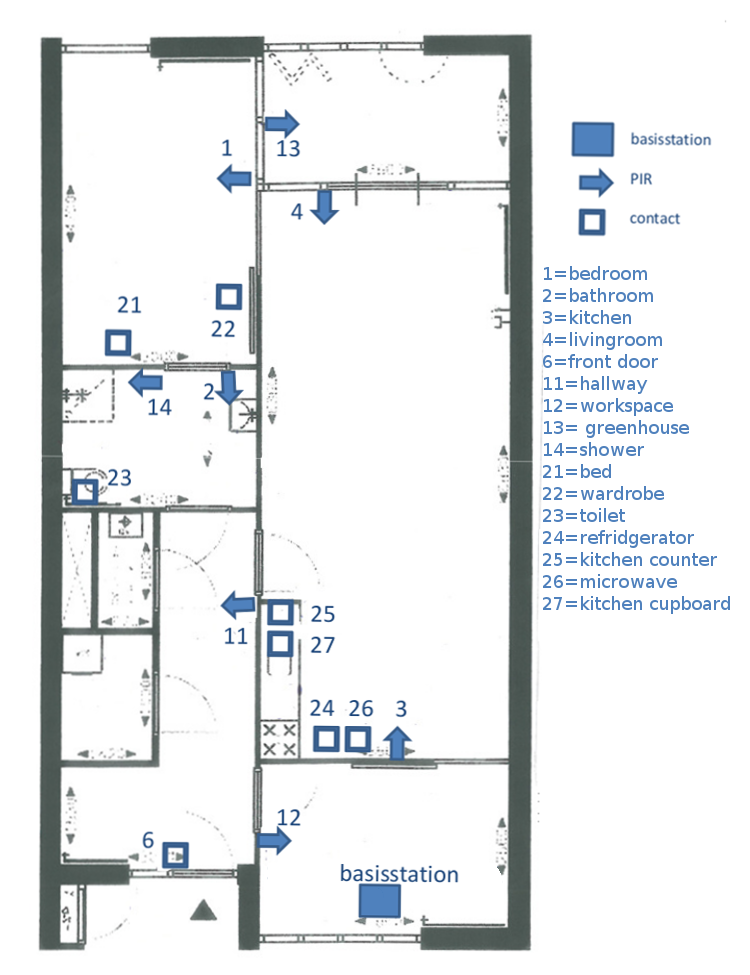
\includegraphics[width=0.7\textwidth]{Pictures/floorplan.png}
 \caption{Floorplan of the houses with sensor descriptions}
 \label{fig:floorplan}
\end{figure}


\begin{table}[h]
\caption{ }
\centering
\begin{tabular}{lccccc}
\centering
HouseNr & 1 & 2 & 3 & 4 & 5 \\
\hline
\# of days & 142 & 98 & 89 & 63 & 73 \\
%time period \\
mean number of events per day & 488 & 523 & 668 & 565 & 427 \\
age & 84 & 77 & 79 & 93 & 95\\
gender & female & female & female & male & female
\end{tabular}
\label{table:houses}
\end{table}




\section{Sensors}
There are different types of sensors installed in the homes. The contact switches are mostly installed at doors and cupboards. They get the value 'one' if a door is opened and the value 'zero' if the door is closed again.
The motion-sensor (PIR) are placed at different places in the homes, mostly against the walls. They have a range of 5 meters. If a motion occurs in the region the sensor sends an impulse value, which means that the value becomes 'one' and immediately 'zero' again . After that the sensor is set to mute for about 3 minutes, which means that in this time there is no motion captured. In this way constantly firing of the sensor will be avoided. The sensor system is active 24 hours and 7 days a week. However failure can occur due to network problems, sensor failing or other unexpected problems.

\section{Received Data}
In figure \ref{fig:PlaineSensorData} the data stream of two different hours of one day is shown. The data belongs to one person. Several sensors that are located in the same room are manually grouped together in a `field'. In the following we use the `fields' $\{$'kitchen', 'living room', 'bathroom', 'bedroom', 'hallway'$\}$. They are marked in the figure with different colors.

\begin{figure}[h!]
   \centering
   \begin{tabular}{c c}
    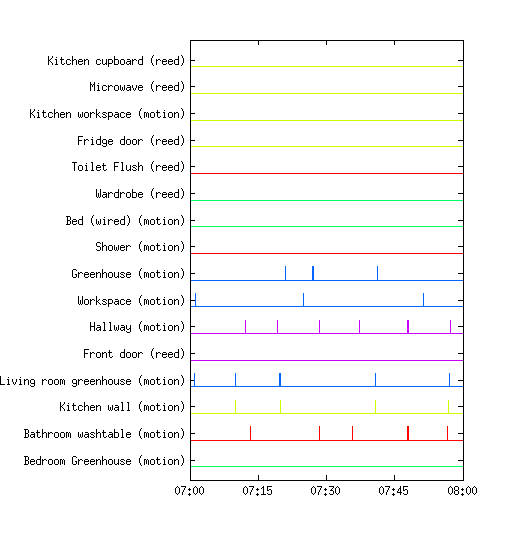
\includegraphics[width=0.45\textwidth]{Pictures/SensorsMorningHN3Day34.png} & 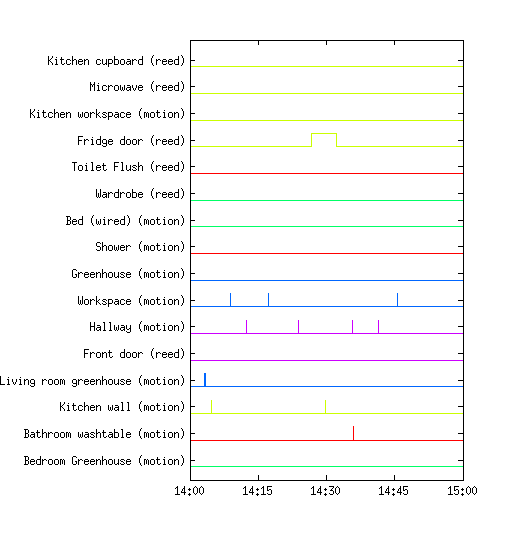
\includegraphics[width=0.45\textwidth]{Pictures/SensorsNoonHN3Day34.png}\\
    a) & b)
   \end{tabular}
   \caption{Sensor Data for two different hours at a day of one person. The fields `kitchen`,'living room','bathroom','bedroom','hallway' are marked with the colors 'yellow', 'blue', 'red', 'green', 'purple' respectively.}
   \label{fig:PlaineSensorData}
 \end{figure}


   

In the figure one can see the different types of data that are generated by the different sensor types. The fridge sensor is a reed sensor which has the value '1' for a longer period of time, when the door is opened for a while. The motion sensors on the other hand only give a impulse value as mentioned before. Some sensors are not triggered at all in the time intervals that are shown.
In the next chapter the feature representation will be described.\\
